%%%%%%%%%%%%%%%%%%%%%%%%%%%%%%%%%%%%%%%%%%%%%%%%%%%%%%%%%%%%%%%%%%
%%%%%%%%%%%%%%%%%%%%%%% Randomer Forest %%%%%%%%%%%%%%%%%%%%%%%%%%
%%%%%%%%%%%%%%%%%%%%%%%%%%%%%%%%%%%%%%%%%%%%%%%%%%%%%%%%%%%%%%%%%%
\documentclass[10pt]{article}
% if you need to pass options to natbib, use, e.g.:
% \PassOptionsToPackage{numbers, compress}{natbib}
% before loading nips_2016
%
% to avoid loading the natbib package, add option nonatbib:
% \usepackage[nonatbib]{nips_2016}

\usepackage[nonatbib]{nips_2016}

% to compile a camera-ready version, add the [final] option, e.g.:
% \usepackage[final]{nips_2016}

\usepackage[utf8]{inputenc} % allow utf-8 input
\usepackage[T1]{fontenc}    % use 8-bit T1 fonts
\usepackage{hyperref}       % hyperlinks
\usepackage{url}            % simple URL typesetting
\usepackage{booktabs}       % professional-quality tables
\usepackage{amsfonts}       % blackboard math symbols
\usepackage{nicefrac}       % compact symbols for 1/2, etc.
\usepackage{microtype}      % microtypography
% \usepackage{fullpage,subfigure,fancyhdr}
\usepackage[pdftex]{color}
\usepackage{wrapfig}
% \usepackage{textcomp}
% \usepackage{verbatim}
% \usepackage{times}
\usepackage{amsmath,amssymb,amsthm}	% math equations, symbols, theorems
\usepackage{mdwlist}	% list-related commands
\usepackage{subfigure}	% subfigures
\usepackage{sidecap}
\usepackage{wrapfig}
\usepackage{xspace}
\usepackage{algorithm,algorithmicx}
\usepackage{algcompatible}
\usepackage[pdftex]{graphicx}
% \usepackage[sort&compress,comma,round,numbers]{natbib}
\usepackage{pict2e}
\usepackage[nottoc,numbib]{tocbibind}
\usepackage{paralist}
\usepackage{multicol}
\usepackage{lettrine}
\usepackage{caption}
\usepackage{helvet}

%%%%%%%%% COMMENTS %%%%%%%%%
\newcommand{\jv}[1]{{\color{magenta}{#1}}}

%%%%%%%%% MATH OPERATORS %%%%%%%%%%%%
\providecommand{\ve}[1]{\boldsymbol{#1}}
\providecommand{\ma}[1]{\boldsymbol{#1}}
\providecommand{\norm}[1]{\left \lVert#1 \right  \rVert}
\providecommand{\deter}[1]{\lvert #1 \rvert}
\providecommand{\abs}[1]{\left \lvert #1 \right \rvert}
\providecommand{\mat}[1]{\left[ #1 \right]}
\newcommand{\trans}[1]{{#1}^{\ensuremath{\mathsf{T}}}}           % transpose
\newcommand{\transpose}[1]{{#1}^{\ensuremath{\mathsf{T}}}}           % transpose
\newcommand{\argmax}{\operatornamewithlimits{argmax}}
\newcommand{\argmin}{\operatornamewithlimits{argmin}}
\newcommand{\T}{^{\ensuremath{\mathsf{T}}}}           % transpose
\newcommand{\from}{{\ensuremath{\colon}}}           % :
\newcommand{\trace}[1]{{\ensuremath{\operatorname{tr}\!\left(#1\right)}}}           % :

\providecommand{\ms}[1]{\mathsf{#1}}
\providecommand{\mc}[1]{\mathcal{#1}}
\providecommand{\mt}[1]{\widetilde{#1}}
\providecommand{\mb}[1]{\boldsymbol{#1}}
\providecommand{\mbb}[1]{\mathbb{#1}}
\providecommand{\mv}[1]{\vec{#1}}
\providecommand{\mh}[1]{\hat{#1}}
\providecommand{\wh}[1]{\widehat{#1}}
\providecommand{\mhv}[1]{\mh{\mv{#1}}}
\providecommand{\mvh}[1]{\mv{\mh{#1}}}
\providecommand{\mhc}[1]{\hat{\mathcal{#1}}}
\providecommand{\mbc}[1]{\mb{\mathcal{#1}}}
\providecommand{\mvc}[1]{\mv{\mathcal{#1}}}
\providecommand{\mtc}[1]{\widetilde{\mathcal{#1}}}
\providecommand{\mth}[1]{\mt{\mh{#1}}}
\providecommand{\mht}[1]{\mh{\mt{#1}}}
\providecommand{\mhb}[1]{\hat{\boldsymbol{#1}}}
\providecommand{\whb}[1]{\widehat{\boldsymbol{#1}}}
\providecommand{\mvb}[1]{\vec{\boldsymbol{#1}}}
\providecommand{\mtb}[1]{\widetilde{\boldsymbol{#1}}}
\providecommand{\mbt}[1]{\widetilde{\boldsymbol{#1}}}
\providecommand{\mvc}[1]{\vec{\mathcal{#1}}}
% \newcommand{\D}[2]{\frac{\partial #1}{\partial #2}}
\newcommand{\dd}[2]{\frac{\partial ^2 #1}{\partial #2 ^2}}
\newcommand{\DDD}[3]{\frac{\partial ^2 #1}{\partial #2 \partial #3}}
\newcommand{\Di}[2]{\frac{\partial ^i #1}{\partial #2 ^i}}

%%%%%% SHORT HAND %%%%%%%%%%
\renewcommand{\refname}{References and Notes}

\newcommand{\Vr}{V_{reset}}
\newcommand{\Vl}{V_{leat}}
\newcommand{\eqdef}{\overset{\triangle}{=}}
\newcommand{\grad}{\nabla}
\newcommand{\Hess}{\nabla\nabla}
\newcommand{\defn}{\overset{\triangle}{=}}

\newcommand{\iid}{\overset{iid}{\sim}}
\newcommand{\knn}{$k$NN}

\newcommand{\elegans}{\emph{C. elegans} }

\newcommand{\Lik}{\mathcal{L}}
\newcommand{\Cae}{[\widehat{\text{Ca}}^{2+}]}
\newcommand{\Cav}{\ve{C}}%[\ve{\text{Ca}}^{2+}]}
\newcommand{\sml}{\sqrt{\ma{\lambda}}}
\newcommand{\ml}{\ma{\lambda}}
\newcommand{\nw}{\widehat{n}}
\newcommand{\nv}{\vec{n}}
\newcommand{\Ae}{\widehat{A}}
\newcommand{\te}{\widehat{\tau}}
\newcommand{\maxn}{\max_{\ve{n}: n_t \geq 0}}
% \newcommand{\V}{\text{Var}}

\newcommand{\PmcP}{P \in \mc{P}}
\newcommand{\mP}{\mathbb{P}}

% \newcommand{\dvs}{\dot{\bs}_t}
% \newcommand{\dvw}{\dot{\bw}_t}
% \newcommand{\dvx}{\dot{\bx}_t}
% \newcommand{\dvy}{\dot{\by}_t}

\newcommand{\ft}{f_{\ve{\thet}}}
\newcommand{\gt}{g_{\ve{\thet}}}
\newcommand{\hht}{h_{\thetn}}

\newcommand{\Real}{\mathbb{R}}


\newcommand{\wconv}{\overset{i.p.}{\rightarrow}}
\newcommand{\sconv}{\overset{i.p.}{\rightarrow}}
\newcommand{\conv}{\rightarrow}
\newcommand{\pconv}{\overset{p}{\conv}}
\newcommand{\mcE}{\mathcal{E}}
\newcommand{\mcT}{\mathcal{T}}
\newcommand{\mcG}{\mathcal{G}}
\newcommand{\mcM}{\mathcal{M}}
\newcommand{\mcL}{\mathcal{L}}
\newcommand{\hatmcE}{\widehat{\mcE}}
\newcommand{\hatp}{\widehat{p}}
\newcommand{\hatP}{\widehat{P}}
\newcommand{\hatQ}{\widehat{Q}}
\newcommand{\hatL}{\widehat{L}}
\newcommand{\mhP}{\widehat{\PP}}
\newcommand{\tildeA}{\widetilde{A}}
\newcommand{\defeq}{\overset{\triangle}{=}}


\DeclareMathOperator{\Pmat}{\mathbf{P}}
\DeclareMathOperator{\veta}{\mathbf{\mb{v}}}
\DeclareMathOperator*{\minimize}{\mathrm{minimize}}
\DeclareMathOperator*{\maximize}{\mathrm{maximize}}
% \DeclareMathOperator*{\mb{v}mod}{\mathbf{\mb{v}}}


%%%%%%% LATIN LETTERS


\newcommand{\bA}{\mb{A}}
\newcommand{\bB}{\mb{B}}
\newcommand{\bD}{\mb{D}}
\newcommand{\bE}{\mb{E}}
\newcommand{\bI}{\mb{I}}
\newcommand{\bP}{\mb{P}}
\newcommand{\bS}{\mb{S}}
\newcommand{\bU}{\mb{U}}
\newcommand{\bV}{\mb{V}}
\newcommand{\bW}{\mb{W}}
\newcommand{\bX}{\mb{X}}
\newcommand{\bY}{\mb{Y}}
\newcommand{\bZ}{\mb{Z}}

\newcommand{\ba}{\mb{a}}
\renewcommand{\ba}{\mb{b}}
\newcommand{\bd}{\mb{d}}
\newcommand{\be}{\mb{e}}
\newcommand{\bp}{\mb{p}}
\newcommand{\bs}{\mb{s}}
\newcommand{\bu}{\mb{u}}
\newcommand{\bv}{\mb{v}}
\newcommand{\bw}{\mb{w}}
\newcommand{\bx}{\mb{x}}
\newcommand{\by}{\mb{y}}
\newcommand{\bz}{\mb{z}}


\newcommand{\Aa}{\mathbb{A}}
\newcommand{\BB}{\mathbb{B}}
\newcommand{\CC}{\mathbb{C}}         
\newcommand{\DD}{\mathbb{D}}         
\newcommand{\EE}{\mathbb{E}}           % expected value
\newcommand{\FF}{\mathbb{F}}         
\newcommand{\GG}{\mathbb{G}}
\newcommand{\HH}{\mathbb{H}}         
\newcommand{\II}{\mathbb{I}}           % indicator function
\newcommand{\LL}{\mathbb{L}}
\newcommand{\MM}{\mathbb{M}}
\newcommand{\NN}{\mathbb{N}}
\newcommand{\PP}{\mathbb{P}}         
\newcommand{\QQ}{\mathbb{Q}}           
\newcommand{\SSS}{\mathbb{S}}           
\newcommand{\VV}{\mathbb{V}}
\newcommand{\WW}{\mathbb{W}}         
\newcommand{\XX}{\mathbb{X}}         
\newcommand{\YY}{\mathbb{Y}}
\newcommand{\ZZ}{\mathbb{Z}}         




\newcommand{\Qs}{Q}
\newcommand{\mcS}{\mc{S}}
\newcommand{\mcU}{\mc{U}}

\newcommand{\mbd}{\mb{d}}
\newcommand{\mbD}{\mb{D}}
\newcommand{\mbx}{\mb{x}}
\newcommand{\mbX}{\mb{X}}
\newcommand{\mby}{\mb{y}}
\newcommand{\mbY}{\mb{Y}}

\newcommand{\mtbd}{\mtb{d}}
\newcommand{\mtbD}{\mtb{D}}
\newcommand{\mtbx}{\mtb{x}}
\newcommand{\mtbX}{\mtb{X}}
\newcommand{\mtby}{\mtb{y}}
\newcommand{\mtbY}{\mtb{Y}}



\DeclareMathOperator{\Ri}{\mathbf{\R}^{-1}}
\DeclareMathOperator{\A}{A}
\DeclareMathOperator{\W}{\mathbf{W}}
\DeclareMathOperator{\V}{\mathbf{V}}
\DeclareMathOperator{\U}{\mathbf{U}}
\DeclareMathOperator{\C}{\mathbf{C}}
\DeclareMathOperator{\uvec}{\mathbf{u}}
\DeclareMathOperator{\D}{\mathbf{D}}
\DeclareMathOperator{\Q}{\mathbf{Q}}
\DeclareMathOperator{\R}{R} %\mathbf{P}}
\DeclareMathOperator{\Y}{\mathbf{Y}}
\DeclareMathOperator{\B}{\mathbf{B}}
\DeclareMathOperator{\Hmat}{\mathbf{H}}
\DeclareMathOperator{\Gmat}{\mathbf{G}}
\DeclareMathOperator{\X}{\mathbf{X}}
\DeclareMathOperator{\Cmat}{C} %\mathbf{L}}\providecommand{\ms}[1]{\mathsf{#1}}

\DeclareMathOperator*{\Ymod}{\mathbf{\Y}}
\DeclareMathOperator*{\Bmod}{\mathbf{B}}
\DeclareMathOperator*{\Hmod}{\mathbf{H}}
\DeclareMathOperator*{\Lmod}{\mathbf{L}}
\DeclareMathOperator*{\Xmod}{\mathbf{\X}}


%%% THETA %%%%

\newcommand{\bth}{\ve{\theta}}
\newcommand{\hth}{\mh{\theta}}
\newcommand{\htth}{\mh{\theta}}
\newcommand{\bhth}{\mh{\ve{\theta}}}
\newcommand{\thetn}{\ve{\theta}}
\newcommand{\thet}{\thetn}
\newcommand{\theth}{\widehat{\ve{\theta}}}
\newcommand{\theto}{\ve{\theta}'}
\newcommand{\wht}{\widehat{\thet}}
\newcommand{\wtt}{\widetilde{\thet}}
\newcommand{\vth}{\ve{\thet}}
\newcommand{\vTh}{\ve{\Theta}}
\newcommand{\hvth}{\widehat{\ve{\thet}}}
\newcommand{\bTh}{\ve{\Theta}}
\newcommand{\hbth}{\widehat{\thet}}
\newcommand{\tbth}{\tilde{\bth}}



% \newcommand{\p}{P_{\bth}}
\newcommand{\pold}{P_{\bth'}}
\newcommand{\pk}{P_{\widehat{\ve{\theta}}^{(k)}}}
\newcommand{\pT}{P_{\thetn_{Tr}}} %\thetn_T
\newcommand{\pO}{P_{\thetn_o}} %\thetn_o
% \newcommand{\Q}{Q(\thetn,\theto)}
% \newcommand{\m}{m^{\ast}}
% \newcommand{\q}{q(\ve{H}_t)}
\newcommand{\Ca}{[\text{Ca}^{2+}]}


%%%%%% GREEK LETTERS

\newcommand{\del}{\delta}
\newcommand{\sig}{\sigma}
\newcommand{\lam}{\lambda}
\newcommand{\gam}{\gamma}
\newcommand{\eps}{\varepsilon}

\newcommand{\Del}{\Delta}
\newcommand{\Sig}{\Sigma}
\newcommand{\Lam}{\Lambda}
\newcommand{\Gam}{\Gamma}

\newcommand{\bSig}{\ve{\Sigma}}
\newcommand{\bOm}{\ve{\Omega}}
\newcommand{\bLam}{\ve{\Lambda}}
\newcommand{\bPhi}{\ve{\Phi}}
\newcommand{\bPsi}{\ve{\Psi}}

\newcommand{\bmu}{\ve{\mu}}
\newcommand{\bal}{\ve{\alpha}}
\newcommand{\bpi}{\ve{\pi}}
\newcommand{\bkap}{\ve{\kappa}}
\newcommand{\bdel}{\ve{\delta}}
\newcommand{\bphi}{\ve{\phi}}
\newcommand{\bpsi}{\ve{\psi}}



\DeclareMathOperator{\Delti}{\mathbf{\Delta}^{-1}}
\DeclareMathOperator{\Delt}{Q} %\mathbf{\Delta}}
% \DeclareMathOperator{\Gam}{\mathbf{\Gamma}}
\DeclareMathOperator{\Gami}{\mathbf{\Gamma}^{-1}}
\DeclareMathOperator{\Sigb}{\mathbf{\Sigma}}






%%%%%%%%%%% ALGORITHM NAMES %%%%%%%%%%%%%


\providecommand{\sct}[1]{{\sc \texttt{#1}}}

\newcommand{\Idt}{\sct{Idt}}
\newcommand{\Svd}{\sct{Svd}}
\newcommand{\Svm}{\sct{Svm}}
\newcommand{\Pca}{\sct{Pca}}
\newcommand{\Fld}{\sct{Fld}}
\newcommand{\Lda}{\sct{Lda}}
\newcommand{\eig}{\sct{eig}}
\newcommand{\Lol}{\sct{Lol}}
\newcommand{\Lal}{\sct{Lal}}
\newcommand{\Qoq}{\sct{Qoq}}
\newcommand{\Lrl}{\sct{Lrl}}
\newcommand{\Lfl}{\sct{Lfl}}
\newcommand{\Faq}{\sct{Faq}}
\newcommand{\qr}{\sct{qr}}

\title{\vspace{-50pt}\db{Randomer Forests}}
\author{Tyler M. Tomita, Mauro Maggioni, Joshua T.~Vogelstein}
\date{}

\begin{document}
\maketitle

\begin{abstract}
Random forest (RF) has been shown to outperform many other classifiers on a variety of datasets, yet its restriction of recursive partitions of the feature space to be axis-aligned is suboptimal in many cases. Several studies have proposed ``oblique'' decision forest methods to address this limitation. However, these methods either aren't well-adapted to problems in which the number of irrelevant features are overwhelming, have a time and space complexity significantly greater than RF, or require additional hyperparameters to be tuned, rendering training of the classifier more difficult. In this work, we establish a generalized forest building scheme, random projection forests. Random forests and many other currently existing decision forest algorithms can be viewed as special cases of this scheme. With this scheme in mind, we propose a special case which we call randomer forests (RerFs). We demonstrate that RerF emprically outperforms RF and another recently proposed oblique forest method in simulations and on benchmark data, and also show that it scales comparably to RF in terms of time and space complexity. Lastly, we propose two augmentations to RerF with the goal of making it more robust to affine transformations and outliers. We conclude that RerF is a competitive alternative to RF and other oblique forests. Open source code will be available. 
\end{abstract} 

\section{Introduction}
\label{intro}

% \paragraph{Opportunity} 
Data science is becoming increasingly important as our ability to collect and process data continues to increase. Supervised learning---the act of using predictors to make a prediction about some target data---is of special interest to many applications, ranging from science to government to industry. Classification, a special case of supervised learning, in which the target data is categorical, is one of the most fundamental learning problems, and has been the subject of much study. A simple pubmed search for the term ``classifier'' reveals nearly 10,000 publications, and a similar arXiv search reports approximately 1000 hits. One of the most popular and best performing classifiers is random forests (RFs) \cite{Breiman2001}. Two recent benchmark papers assess the performance of many different classification algorithms on many different datasets \cite{Delgado2014,Caruana2008}, and both concluded the same thing: RFs are the best classifier.

% \paragraph{Challenge}
RF typically refers to Breiman's Forest-IC, which uses axis-parallel \cite{Heath1993}, or orthogonal trees \cite{Menze2011}. That is, the feature space is recursively split along directions parallel to the axes of the feature space. Thus, in cases in which the classes seem inseparable along any single dimension, RF may be suboptimal. To address this, Breiman also proposed and characterized Forest-RC, which used linear combinations of coordinates rather than individual coordinates, to split along. Others have studied several different variants of ``oblique'' decision forests, including efforts to learn good projections \cite{Heath1993,Tan2005}, using principal components analysis to find the directions of maximal variance \cite{Ho1998,Rodriguez2006}, or directly learning good discriminant directions \cite{Menze2011}. Another recently proposed method, called random rotation RF, uniformly randomly rotates the data for every decision tree in the ensemble prior to inducing the tree \cite{Blaser2015}. While all of these recent approaches deal with rotational invariance, they fail to address two important issues. First, in real world data, the proportion of features that are irrelevant is often large, especially for high dimensional data, giving rise to optimal decision boundaries that are sparse. In such cases, we say that the signal is \textit{compressive}. To our knowledge, all of the proposed oblique decision forests, with the exception of Forest-RC if tuned appropriately, do not impose a constraint on the sparsity of recursive partitions of the feature space. Therefore, such methods may be suboptimal in cases in which the signal is compressive. Second, as our ability to collect and process data continues to increase, we are encountering increasingly massive datasets. Therefore, time- and space-efficient methods are becoming more and more important. With the exception of Forest-RC, all oblique methods require expensive computation and/or storage. There is therefore a gap that calls for the construction of a scalable oblique decision forest classifier that can perform well in the presence of an overwhelming number of irrelevant features. It is true that Forest-RC fits this description. However, the number of features that are linearly combined to generate candidate splits is fixed across all nodes of every tree. Such a construction requires an additional hyperparameter to be tuned, and also limits the diversity of trees. 

% \paragraph{Action}
To address this, we first state a generalized forest building scheme, random projection forests, which includes all of the above algorithms as special cases. This enables us to formally state our objective, and provides a lens that enables us to propose a few novel special cases, which we refer to as ``{\em{Randomer Forests}}'' (or RerFs for short), for reasons that will become clear in the sequel. We both theoretically and empirically demonstrate that our methods have the same time and space complexity as random forests, and show on simulated datasets that it performs well in the face of many irrelevant features and when axis-aligned splits are suboptimal. Additionally, we demonstrate that our method empirically outperforms both RF and random rotation RF (RotRF), which is another oblique method \cite{Blaser2015}, on a suite of benchmark datasets. Lastly, we propose two augmentations to RerF for making the method more robust to affine transformations and outliers. To conclude, we propose our method as a competitive alternative to RF and other oblique decision forest methods. Open source code will be made available.

\section{Random Projection Forests}

Let $\mc{D}^n=\{(X_i,y_i): i \in [n]\}$ be a given dataset, where $X_i \in \Real^p$ and $y_i \in \mc{Y} = \{\mt{y}_1,\ldots, \mt{y}_C\}$. A classification forest, $\bar{g}(X; \mc{D}^n)$ is an ensemble of $L$ decision trees, each tree $g^l( X; \mc{D}^l)$ is trained on a (sub)set of the data, $\mc{D}^l \subset \mc{D}^n)$.
Random Projection forests are a special case of classification forests that subsume all of the strategies mentioned above (see Pseudocode \ref{pseudo}). The key idea of all of them is that at each node of the tree, we have a set of predictor data points, $\bar{X}=\{X_s\}_{s \in \mc{S}^l_{ij}} \in \Real^{p \times S^l_{ij}}$ , where  $S^l_{ij}=|\mc{S}^l_{ij}|$ is the cardinality of the set of predictor data points at the $(ij)^{th}$ node of the $l^{th}$ tree.
We sample a matrix $A \sim f_A(\mc{D}^n)$, where $A \in \Real^{p \times d}$, possibly in a data dependent fashion, which we use to project the predictor matrix $\bar{X}$ onto a lower dimensional subspace, yielding $\mt{X} = A\T X \in \Real^{d \times S^l_{ij}}$, where $d \leq p$ is the dimensionality of the subspace. To wit, Breiman's original Forest-IC algorithm can be characterized as a special case of random projection forests. In particular, in Forest-IC one constructs $A$ such that for each of the $d$ columns, we sample a coordinate (without replacement), and put a 1 in that coordinate, and zeros elsewhere. Breiman's Forest-RC constructs $A$ by sampling a fixed number of coordinates (without replacement) for each of the $d$ columns, and puts a value uniformly sampled from [-1,1] in each of those coordinates. Similarly, Ho's rotation forests construct $A$ from the top $d$ principal components of the data $\bar{X}$ at a given node. Thus, the key difference in all these approaches is the choice of $f_A$. 

\begin{algorithm}
  \caption{Psuedocode for Random Projection Forests, which generalizes a wide range of previously proposed decision forests.}
  \label{pseudo}
\begin{algorithmic}
  \STATE {\bfseries Input:} data: $\mc{D}^n = (X_i,y_i) \in (\Real^p \times \mc{Y})$ for $i \in [n]$, tree rules (stopping criteria, rules for sampling data points per tree, etc.), distributions on $d \times p$ matrices}: $A \sim f_A(\mc{D}^n)$, preprocessing rules
  \STATE {\bfseries Output:} decision trees, predictions, out of bag errors, etc. 
  \STATE Preprocess according to rule
  \FOR{each tree}
  \STATE Subsample data to obtain $(\bar{X},\bar{y})$, the set of data points to be used in this tree
  \FOR{each leaf node in tree}
  \STATE Let $\mt{X} =  A\T \bar{X} \in \Real^{d \times s}$, where $A \sim f_A(\mc{D}^n)$
  \STATE Find the ``best'' split coordinate $k^*$ in $\mt{X}$ and ``best'' split value $t^*(k^*)$ for this coordinate
  \STATE Split $X$ according to whether $X(k) > t^*(k^*)$
  \STATE Assign each child node as a leaf or terminal  node according to stopping criteria
  \ENDFOR
  \ENDFOR
  \STATE Prune trees according to rule
\end{algorithmic}
\end{algorithm}

The goal of this work is to find a random projection forest that shares RF's scalability and ability to perform well when many irrelvant predictors are present, yet is able to find decision boundaries that are less biased by geometrical constraints (i.e. not constrained to be axis-aligned), by changing the distribution $f_A$. The result we call randomer forests (or RerFs for short).

\section{Randomer Forests}

Our choice in $f_A$ is based on the following three ideas:
\begin{enumerate}
  \item While RF empirically performs well in many settings, it is quite restrictive in that candidate splits evaluated at each node are constrained to be axis-aligned. It is sometimes the case that axis-aligned splits are suboptimal, and oblique splits may be desired.
  \item It is often the case that the number of \textit{relevant} features is substantially smaller than the number of total features. We say that the signal is \textit{compressive} in such cases. RF often does well when the signal is compressive, which may be attributed, in part, to the extreme sparsity constraint on the columns of A. All of the oblique decision forest algorithms to date, with the exception of Forest-RC, do not impose a sparsity constraint on the candidate split directions, which may cause such algorithms to underperform when the signal is compressive.
  \item Except for Breiman's Forest-RC, existing oblique decision forest algorithms involve expensive computations to identify and select splits, rendering them less space and time efficient than Forest-IC or Forest-RC. An oblique decision forest having a space and time complexity comparable to Forest-IC or Forest-RC is desirable.
\end{enumerate}

To this end, we employ very {\bf{sparse random projections}} \cite{Li2006}. Rather than sampling $d$ non-zero elements of $A$ and enforcing that each column gets a single non-zero number (without replacement) as RF does, we relax these constraints and select $d$ non-zero numbers from $\{-1,+1\}$ with equal probabilities and distribute uniformly at random in $A$.

It is apparent that RerF bares a resemblance to Forest-RC, yet there is one key difference. In Forest-RC, the number of nonzeros in each column of $A$ is fixed to be the same across $A$ and for every split node, and its optimal value has to be found through parameter selection. Our construction circumvents selection of this parameter by randomizing the number of nonzeros in each column of $A$. Furthermore, our algorithm allows $A$ to have columns of varying sparsity, which may promote more diversity in the ensemble. To our knowledge, this property does not exist in any of the proposed random projection forest algorithms. Lastly, we note that our construction of $A$ preserves distances between points with high probability \cite{Li2006}.

\section{Experimental Results}

\subsection{Simulations Involving Compressive Signals}
\label{section: sims}

Many classification problems arise in which the signal is compressive and the optimal split directions are not axis-aligned. We constructed two synthetic datasets with both of these properties to compare classification performance and training time of RF, RerF, and RotRF:
% \begin{compactenum}

\textbf{Sparse parity} is a variation of the noisy parity problem. The noisy parity problem is a multivariate generalization of the noisy XOR problem and is one of the hardest constructed binary classification problems. In the noisy parity problem, a given sample has a mean whose elements are Bernoulli samples with probability 1/2, and then Gaussian noise is independently added to each dimension with the same variance.  A sample's class label is equal to the parity of its mean. Sparse parity is an adaption of this problem in which the sample's class label is equal to the parity of only the first $p*$ elements of the mean, rendering the remaining $p - p*$ dimensions as noise.

\textbf{Trunk} is a well-known binary classification in which each class is distributed as a p-dimensional multivariate Gaussian with identity covariance matrices \cite{Trunk1979}. The means of the two classes are $\mu_1 = (1,\frac{1}{\sqrt{2}},\frac{1}{\sqrt{3}},...,\frac{1}{\sqrt{p}})$ and $\mu_2 = -\mu_1$. It follows from this that the signal-to-noise ratio of the $ith$ dimension asymptotically decreases to zero with increasing $i$.

RotRF is an oblique decision forest method that has been recently proposed in \cite{Blaser2015}. RotRF works exactly like RF, except that the feature space is uniformly randomly rotated prior to inducing each decision tree. This induces oblique splits in an unstructured way, which the authors argue is favorable to structured methods such as in Rodriguez's rotation forest, because such structured methods reduce the diversity of the trees. Uniformly random rotations of the feature space imply that in general, splits will not be sparse. Therefore, we conjecture that RotRF will perform increasingly poorly as the ratio of the number of irrelevant features to the number of relevant features becomes larger, while RF and RerF will be relatively more robust to the increasing presence of irrelevant features.

Figure \ref{posteriors} depicts the true class posteriors in the first two dimensions of the sparse parity simulation in panel A and estimates of the posteriors for RF, RerF, and RotRF in panels B, C, and D, respectively. For this simulation, $p = 20$, $p* = 3$, and $n = 1000$, where $p$ is the total number of dimensions, $p*$ is the number of relevant dimensions, and n is the number of sampled data points. The number of trees used for all three algorithms was 1000. Various values of $d$, the number of columns in the random projection matrix $A$, were tried and the best for each algorithm was selected. RerF gives estimates of the posteriors closest to the true posteriors. 

\begin{figure}[ht]
\vskip 0.2in
\begin{center}
\centerline{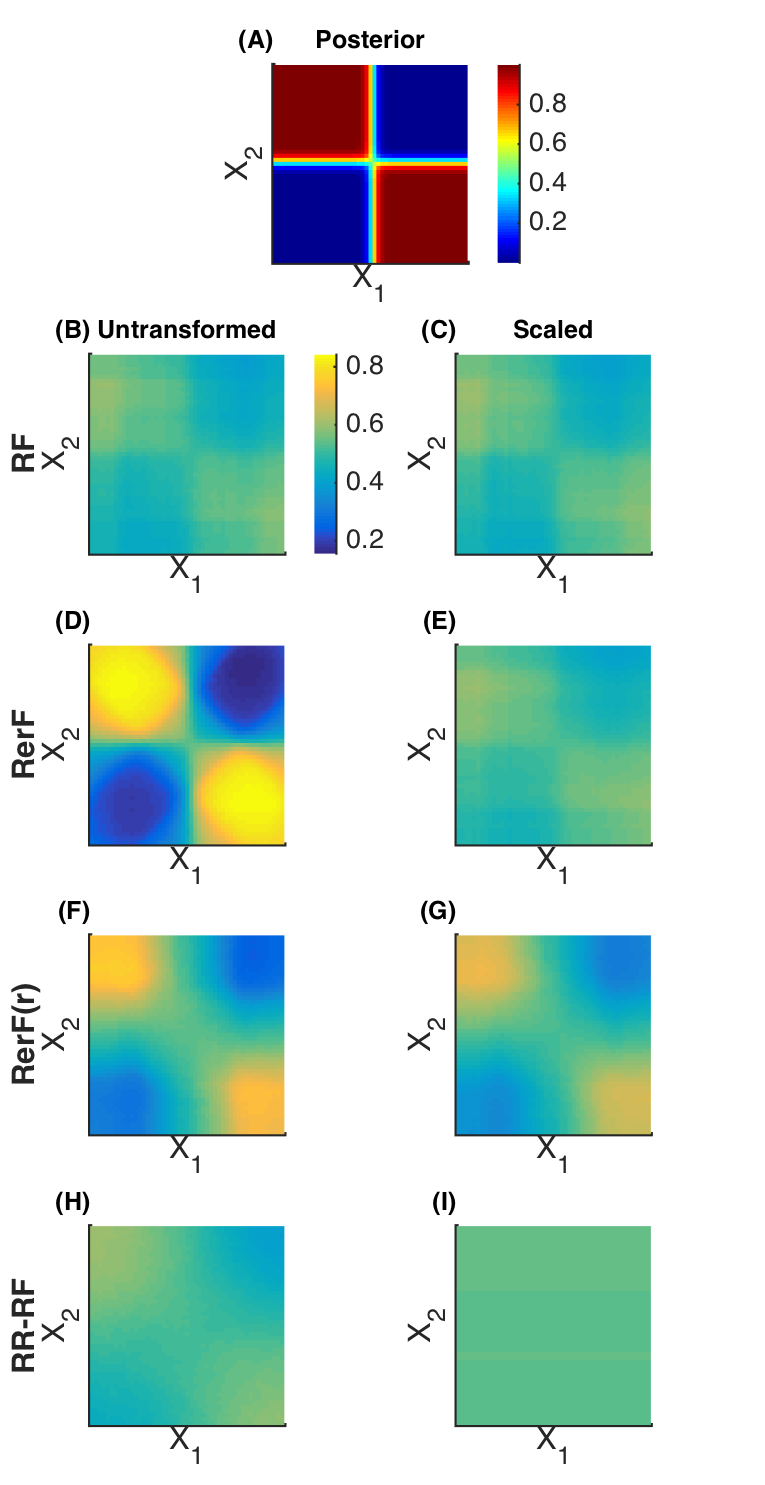
\includegraphics[width=\columnwidth]{../Figures/pdf/Sparse_parity_posteriors}}
\caption{Class posteriors for the sparse parity problem in the first two dimensions (refer to section \ref{section: sims} for details). (A): True posteriors. (B) - (D): Posterior estimates for RF, RerF, and RotRF, respectively. Comparing panels B-D with A, it is evident that RerF produces better estimates of the posteriors than does RF or RotRF}
\label{posteriors}
\end{center}
\vskip -0.2in
\end{figure}

The left panels of Figure \ref{simulations} show two-dimensional scatter plots from each of the two example simulations (using the first two coordinate dimensions). The middle panels show the misclassification rate relative to RF against the number of observed dimensions $p$, for RerF and RotRF. Relative misclassifcation rate was computed as the difference between the misclassification rate of either RerF or RotRF and that of RF. The misclassification rate of RF relative to itself is shown for reference. The right panels show training time against the number of observed dimensions $p$ for all four classifiers. For all comparisons, we used the same number of trees for each method to enable a fair comparison. The number of trees used for each method in the sparse parity and Trunk simulations were 500 and 1000, respectively. In all methods, trees were pruned and the minimum number of data points at a node in order to be considered for splitting was 10. Gini impurity was used as the split criteria. The only parameter tuned was $d$, the number of candidate split directions evaluated at each split node. When $p \leq 5$, each classifier was trained for all $d \in [p]$. When $p > 5$, each classifier was trained for all $d \in \{1,p^{1/4},p^{1/2},p^{3/4},p\}$. Misclassification rates for each classifier were selected as the lowest achieved from the different values of $d$ tried. Training times for each classifier were computed by averaging the training times given by all values of $d$ tried. For sparse parity, $n$ was fixed at 1000 and classifiers were evaluated for $p \in \{2,5,10,25,50,100\}$. The relevant number of features $p*$ was fixed at a value of 3. For Trunk, $n$ was fixed at 100 and RF and RerF were evaluated for $p \in \{2,10,50,100,500,1000\}$. RotRF was not evaluated for $p = 1000$ due to computational burden. Relative error and training times plotted are the average of 25 repeated trials, and error bars represent the standard error of the mean.

In panel B, RerF performs as well as or better than both RF and RotRF for all values of $p$. RotRF performs as well as or better than RF except for when $p = 25$. As conjectured, RotRF performs better than RF when $p$ is small because oblique splits provide an advantage over axis-aligned splits in the sparse parity problem. As $p$ increases and the ratio $p*/p$ decreases, RerF begins to outperform RotRF. Ultimately, when this ratio is small enough, RotRF performs even worse than RF. RerF's ability to perform relatively well can be attributed to the sparsity of oblique splits. In panel E, RerF outperforms RF for all values of $p$. This is because linear combinations of a few features can yield a higher signal-to-noise ratio than any single feature. RotRF outperforms both RF and RerF up to $p = 100$. RotRF is able to perform better than RerF in these cases because a larger number of features can be linearly combined to yield an even higher signal-to-noise ratio. When $p = 500$, classification performance of RotRF significantly degrades and becomes worse than both RF and RerF. This can be explained by the fact that when $p$ is large enough, RotRF often samples linear combinations of many features each having a low signal-to-noise ratio. Such projections will yield a lower signal-to-noise ratio than any single feature. In panels C and F, training times are comparable when $p$ is small. As panel F indicates, training time of RotRF is significantly longer than those of RF and RerF when $p = 500$. 

\begin{figure}[ht]
\vskip 0.2in
\begin{center}
\centerline{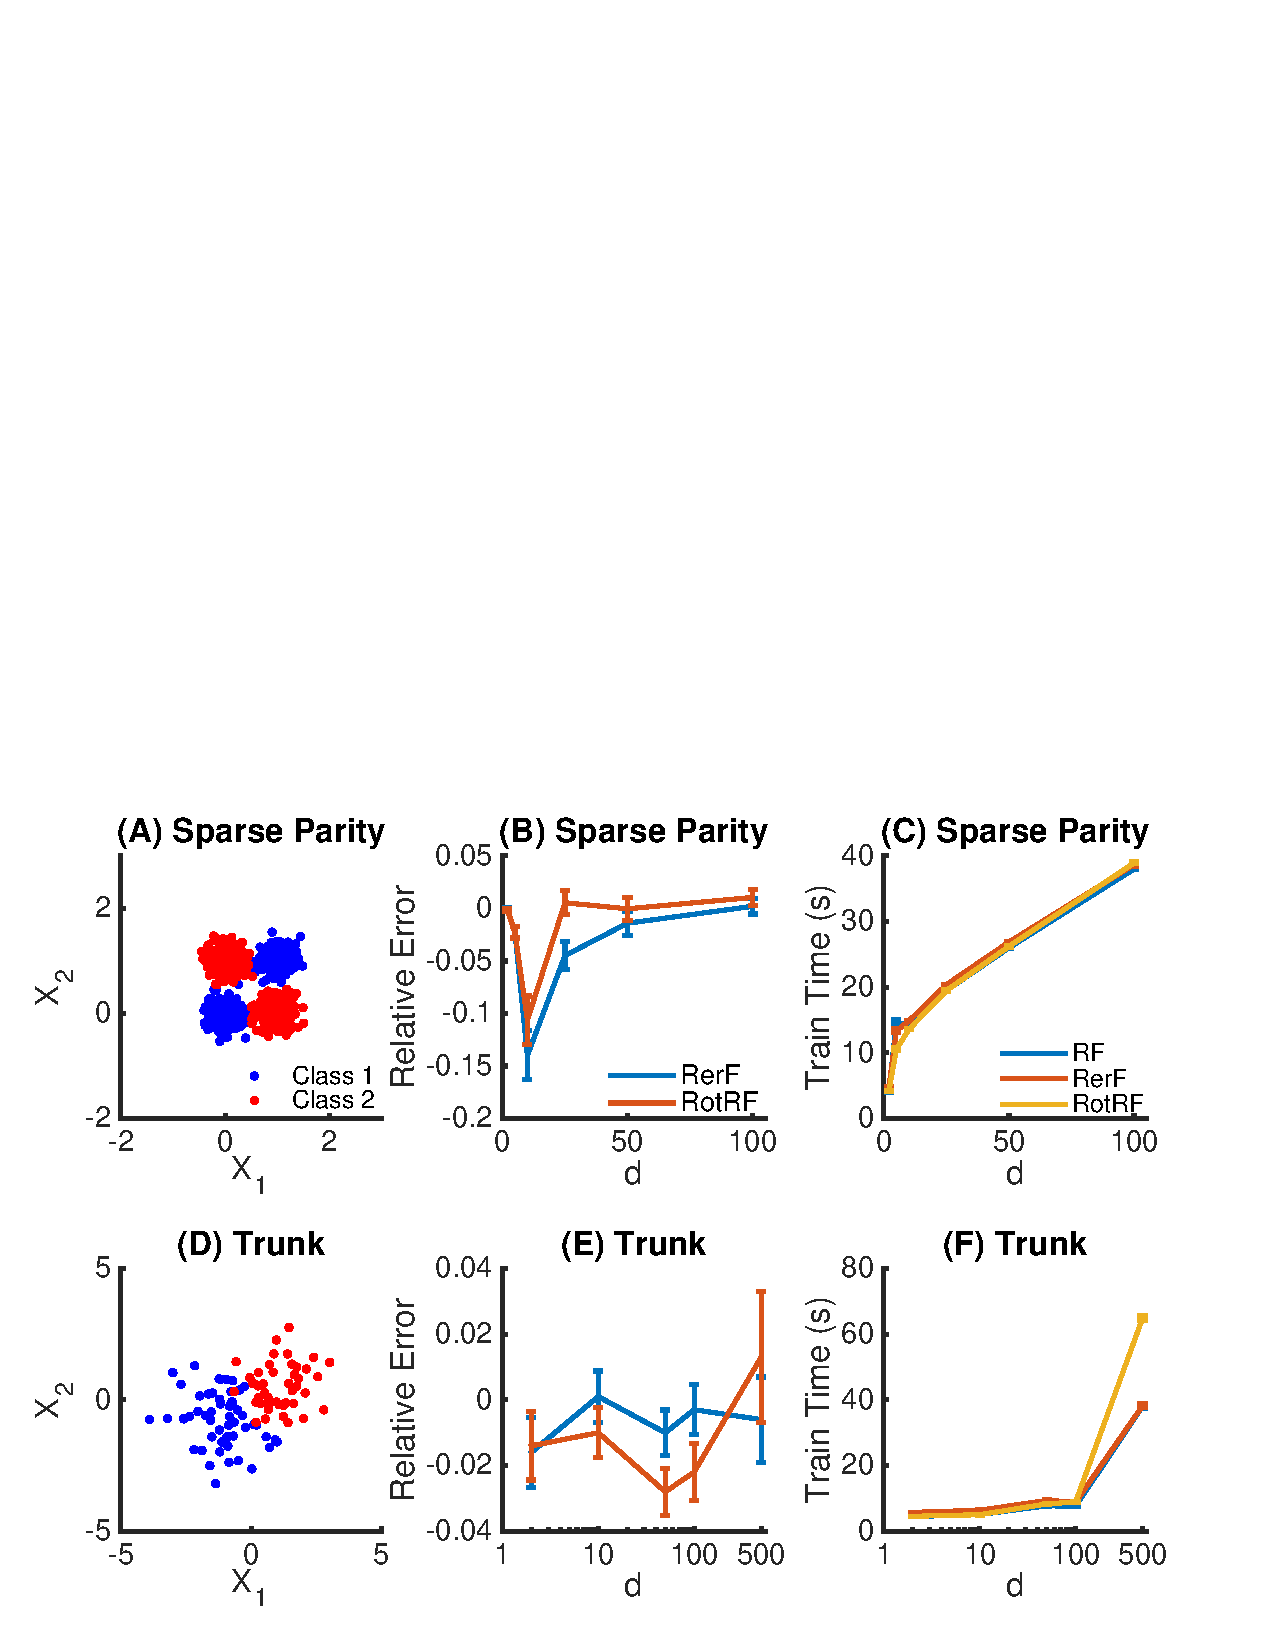
\includegraphics[width=\columnwidth]{../Figures/pdf/Fig2_simulations}}
\caption{Sparse parity (A-C) and Trunk (D-F) simulations (see section \ref{section: sims} for details). (A) and (D): Scatterplots of sampled points in the first two dimensions. (B) and (E): Error rates of RerF and RotRF relative to RF across different values of p. (C) and (F): Same as (B) and (E) except absolute training time is plotted on the y-axis instead. The cyan, green, and magenta lines correspond to RF, RerF, and RotRF, respectively. This color coding is adopted in figures \ref{transformations} and \ref{benchmark} that follow. Both RerF and RotRF do better than RF when the number of irrelevant features is sufficiently small, due to their ability to generate oblique parititions. However, when the number of irrelevant features becomes large enough, performance of RotRF rapidly degrades. Training times show that RerF scales identically with RF, while RotRF scales poorly with large p (note that in panels E and F, RotRF is only plotted up to $p = 500$ due to computational constraints.}
\label{simulations}
\end{center}
\vskip -0.2in
\end{figure}

\subsection{Theoretical Space and Time Complexity}

For a RF, assume there are $L$ trees.  
If there are $n$ data points per tree, and each tree grows until terminal nodes have only $\mc O(1)$ data points with $p$ coordinates in them, there are $\mc O(n)$ nodes.
Then the complexity of constructing the random forest, disregarding cross-validation or other randomization techniques for preventing overfitting, is $\mc O(Ln^2p\log n)$. In practice the trees are shallower and stop much earlier than when nodes have $\mc O(1)$ points, so ``in practice'' the complexity often appears to be $\mc O(Lnp\log n)$. Storing RF requires $\mc{O}(L n\log n )$ because each node can be represented by the index of the nonzero coordinate. The only additional space constraint is storing which indices are positive, and which are negative, which is merely another constant.

RerF has a very similar time and space complexity, unlike many of the other oblique random forest variants.  Specifically, assume that RerF also has $L$ trees, and $n$ data points per tree, and no pruning, so $\mc O(n)$ nodes. Let $n_k$ be the number of data points at node $k$ of the tree. Like RF, RerF requires $\mc{O}(p)$ time to sample $p$ non-zero numbers, and $\mc{O}(pn_k)$ time to obtain the new matrix, $\mt{X}$, because it is a sparse matrix multiplication, in node $k$ with $\mc O(n_k)$ points. RerF also takes another $\mc{O}(p/n\log(p/n))=\mc O(1)$ time to find the best dimension. Thus, in total, in the case of well-balanced trees, RerF also requires only $\mc{O}(Lpn^2\log n)$ time to train.  To store the resulting RerF, like RF, requires $\mc{O}(L n\log n )$, because each node can be represented by the indices of the coordinates that received a non-zero element, and the expected number of such indices is $\mc O(1)$. Note that these numbers are in stark contrast to other oblique methods. RotRFs, in particular, require a QR decomposition having a time complexity of $\mc O(p^3)$ in order to generate random rotation matrix for each tree. Rotating the data matrix prior to inducing each tree additionally requires $\mc O(np^2)$. Therefore, RotRF becomes very expensive to compute when $p$ is large. This can explain the trend seen in Figure \ref{simulations}(F). In addition to storing all of the decision trees, RotRF has to store a rotation matrix for each tree, which requires $\mc O(p^2)$.

\subsection{Effects of Transformations and Outliers}
\label{section: trans}

We next want to compare the robustness of RF, RerF, and RotRF to various data transformations. To do so, we consider several different modifications to the simulation settings described in the previous section: rotation, scale, affine, and outliers.  To rotate the data, we simply generate rotation matrices uniformly and apply them to the data. To scale, we applied a scaling factor sampled from a uniform distribution on the interval [0,10] to each dimension. Affine transformations were performed by applying a combination of rotations and scalings as just described. Additionally, we examined the effects of introducing outliers. Outliers were introduced by sampling points from the distributions as previously described but instead using covariance matrices scaled up by a factor of four. Empirically, an addition of 20 points from these outlier models to the original 100 points was found to produce a noticeable but not overwhelming effect on classifier performance.

Figure \ref{transformations} shows the effect of these transformations and outliers on the sparse parity (panels A-E) and Trunk (panels F-J) problems. Panels A-E show that RerF and RotRF outperform RF in both untransformed and transformed representations for Sparse Parity. This makes sense because linear combinations of variables can have some information about the class, whereas the original features are all uninformative on their own. For the trunk simulations, panel G shows that RotRF is more robust to rotations (as it should be), but is fragile in the face of affine transformations.

\begin{figure}[ht]
\vskip 0.2in
\begin{center}
\centerline{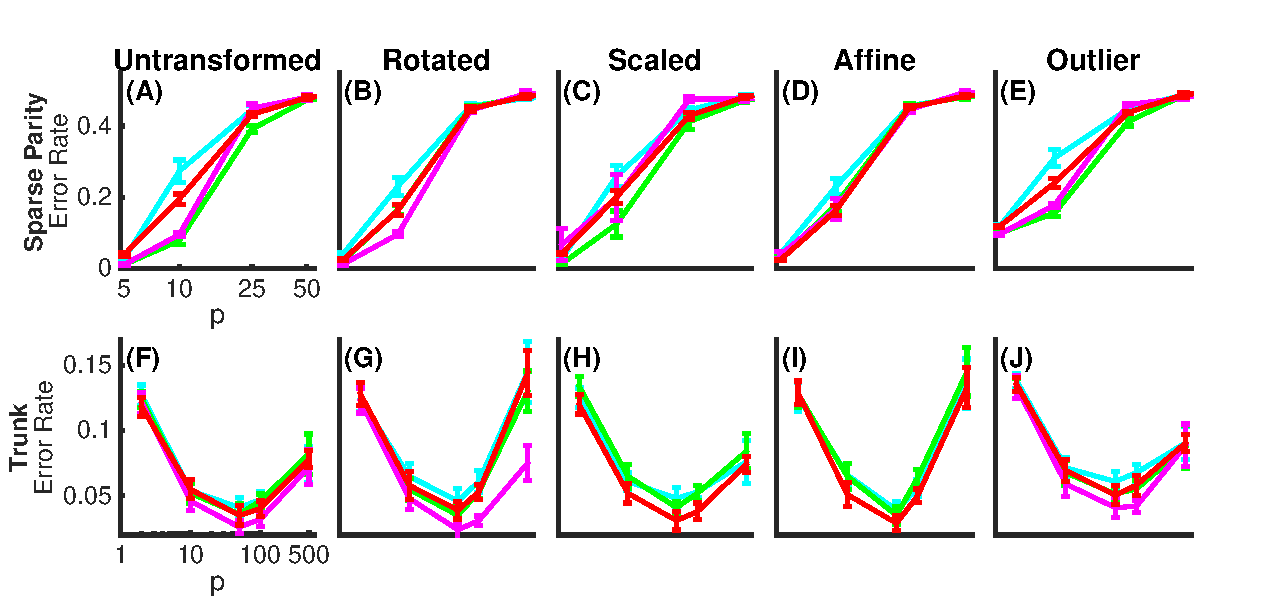
\includegraphics[width=\columnwidth]{../Figures/pdf/Fig3_transformations2}}
\caption{The effects of different transformations applied to the sparse parity (A-E) and Trunk (F-J) simulations on classification performance (see section \ref{section: trans} for details). Specifically, we consider rotations, scalings, affine transformations, as well as the addition of outliers. RerF and RotRF outperform RF on sparse parity. The trunk simulations demonstrate clearly that RotRF, while invariant to rotation, is sensitive to affine transformations.}
\label{transformations}
\end{center}
\vskip -0.2in
\end{figure}

\subsection{Benchmark Data}
\label{section: benchmark}

In addition to the simulations, RF, RerF, and RotRF were evaluated on 115 of the 121 datasets as described in \cite{Delgado2014}. The six remaining datasets were not used because their high dimensionality and large number of data points rendered the classifiers both time and space costly, particularly for RotRF. As in the previous section, transformations, with the exception of outliers, were applied to the datasets to observe their affects on performance of the three algorithms. Classifiers were trained on the entire training sets provided. For each data set, misclassification rates were again estimated by out of bag error. The number of trees used in each algorithm was 1000 for datasets having at most 1000 data points and 500 for datasets having greater than 1000 data points. All algorithms were trained using five different values for $d$, and error rates for each algorithm were selected as the minimum given by the five. For each dataset, relative performance ratios for each algorithm were computed by dividing the error rate of each algorithm by the minimum error rate of the three. The empirical cumulative distribution functions of relative performance ratios for each algorithm were computed and plotted in panels A-D of Figure \ref{benchmark}. Such plots are called performance profiles \cite{Dolan2002}. Performance profiles are useful in visualizing how frequently a particular algorithm wins, and when it loses, how frequently it loses by a certain amount. Areas under the curves (AUCs) were computed for each performance profile. This metric is valuable in that it doesn't necessarily indicate how frequently a particular algorithm is the best. Rather, it is an indicator of robustness. For instance, it is possible that an algorithm that wins on the majority of datasets can have a lower AUC than the other algorithms if, when it loses, it frequently loses by a large margin. On the original benchmarks (Figure \ref{benchmark} panel A), RerF achieves the largest AUC, followed by RF and lastly RotRF. The same trend is seen when scaling (panel C) and affine transformations (panel D) are applied. When the datasets are rotated, RotRF achieves the largest AUC, followed by RerF, and lastly RF.

Since the simulations in section \ref{section: sims} revealed that the speed of RF and RerF scaled comparably, we wanted to see if this observation held on the benchmark data. In the same fasion as the left panels of Figure \ref{benchmark}, we plotted performance profiles for training times in the right panels. Across all transformations, we see that RF and RerF perform comparably in terms of speed. Panels A and C show that RotRF performs the worst on the original benchmark data and the randomly scaled benchmark data. It performs well, however, on the rotated and affine transformed data. One possible explanation for this is that when the data is rotated, RF and RerF have a more difficult time finding good split directions, which could result in deeper trees (and subsequently more time spent in training).  

\begin{figure}[ht]
\vskip 0.2in
\begin{center}
\centerline{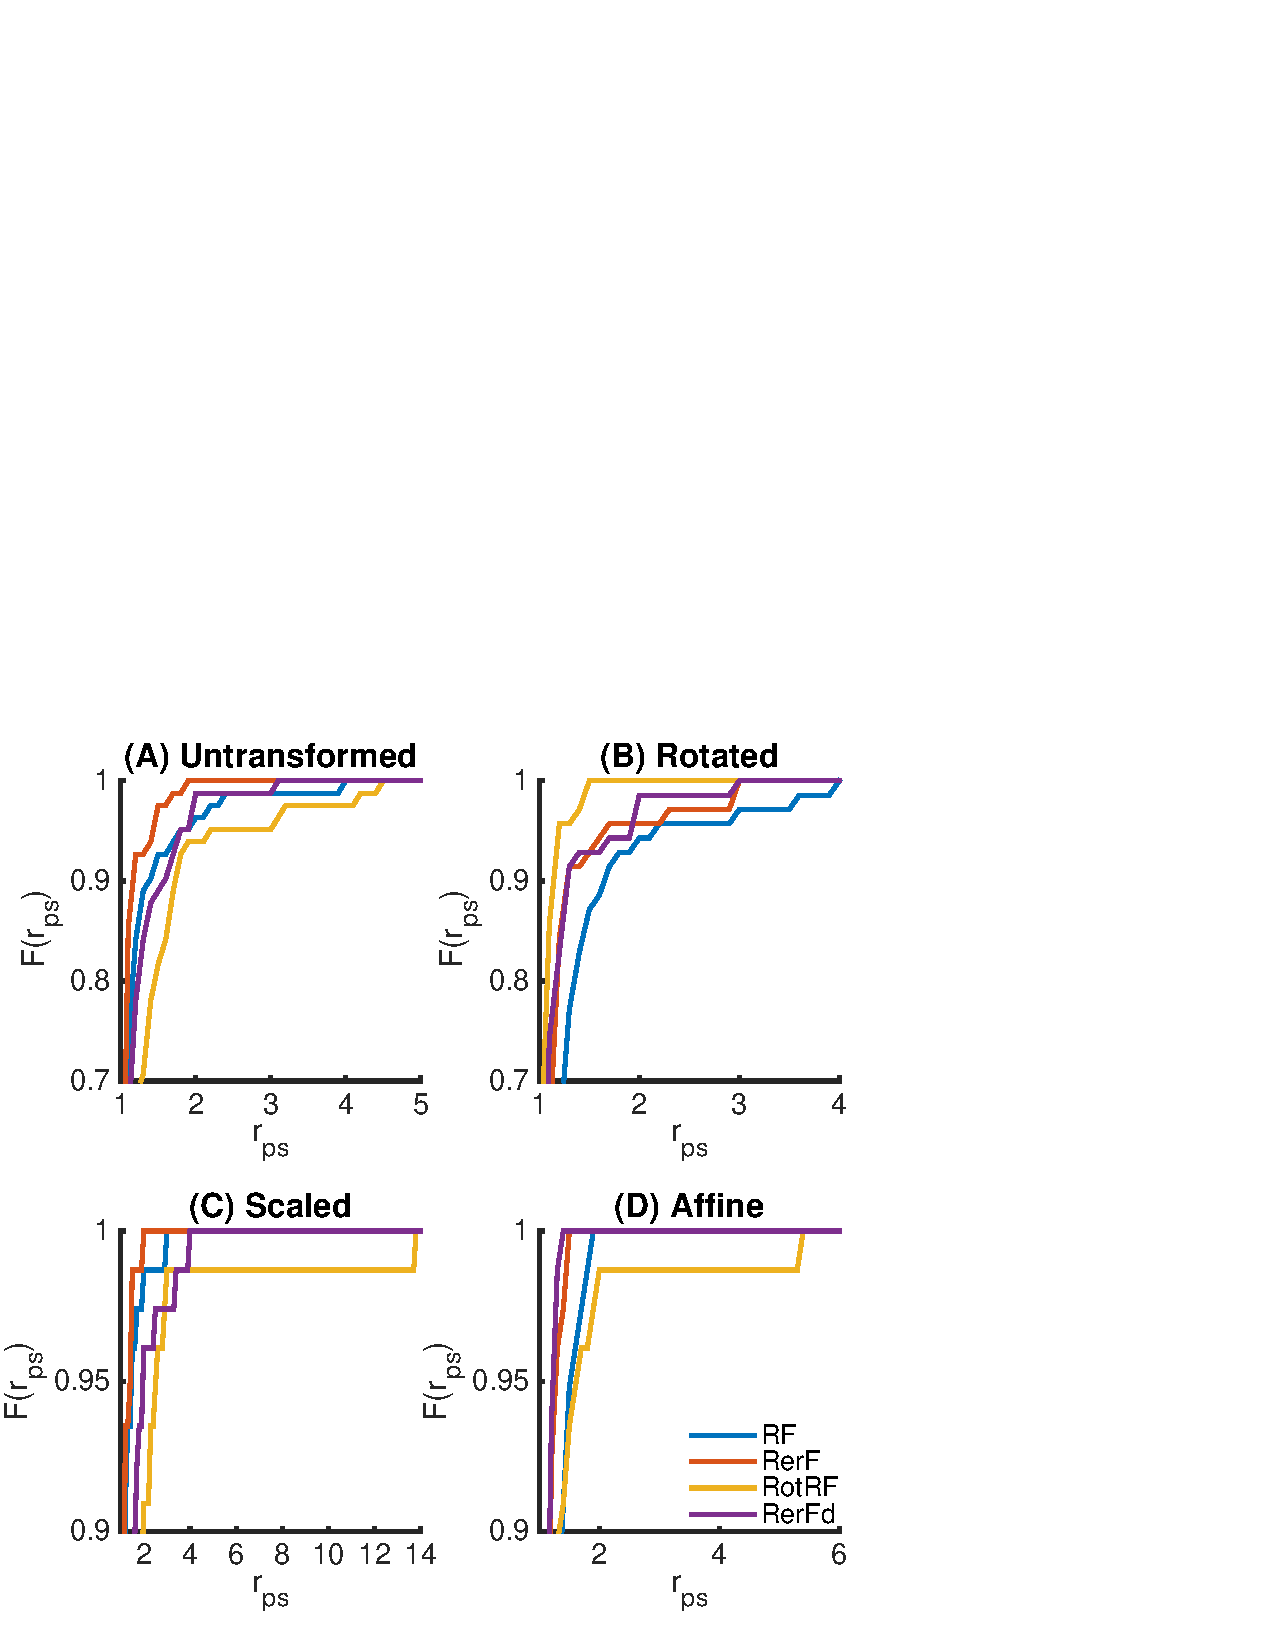
\includegraphics[width=\columnwidth]{../Figures/pdf/Fig4_benchmark}}
\caption{Classification (panels A-D) and speed (panels E-H) performance profiles on benchmarks with various transformations applied (see section \ref{section: benchmark} for details). AUC denotes the area under the curve. In terms of classification accuracy, RerF outperforms RF in all five data settings and only loses to RotRF when the data is rotated. RF and RerF have comparable training time performance, while RotRF tends to be slower.}
\label{benchmark}
\end{center}
\vskip -0.2in
\end{figure}

\subsection{Rank Transforming the Data and Fast Supervised Projections}
\label{section: additions}

When dimensions of $X$ are linearly combined, we lose {\em{scale and unit invariance}}. We therefore note that random forests have a special property: they are invariant to monotonic transformations of the data applied to each coordinate in the ambient (observed) space. They are effectively operating on the order statistics, rather than actual magnitudes of coordinates. In other words, if we convert for each dimension the values of the samples to their corresponding ranks, random forests yield the exact same result. Therefore, for our second trick, we adopt the same policy, and ``{\bf{pass to ranks}}'', or rank transform,  prior to doing anything else. We call RerFs that pass to ranks RerF(r).

Additionally, there is evidence that {\em{using the data to construct $A$ at each node}} can significantly improve performance \cite{Heath1993}. However, previously proposed approaches for using the data require methods that are time- and space-intensive compared to standard random forests.  We propose a simple strategy: ``{\bf{compute the mean difference vectors}}''. In other words, given a two-class problem, let $\mh{\delta}=\mh{\mu}_0-\mh{\mu}_1$, where $\mh{\mu}_c$ is the estimated class conditional mean. Under a spherically symmetric class conditional distribution assumption, $\mh{\delta}$ is the optimal projection vector. When there are $C>2$ classes, the set of all pairwise distances between $\mh{\mu}_c$ and $\mh{\mu}_{c'}$ is of rank $C-1$. Because RerFs are approximately rotationally invariant, we can simply compute all the class conditional means, and subtract each from one of them (we chose the $\mh{\mu}_c$ for which $n_c$, the number of samples in that class, is the largest). Thus, we construct $\mt{X}$ by concatenating $A\T$ with $\Delta=(\delta_{(2)} - \delta_{(1)}, \ldots, \delta_{(C)} - \delta_{(1)})$, where $\delta_{(j)}$ is the $\delta$ vector for the class with the $j^{th}$ largest number of samples, to obtain $\mt{A}\T$. Then we compute $\mt{X} = \mt{A}\T\bar{X}$. Computing this matrix is extremely fast, because it does not rely on costly singular value decompositions, matrix inversions, or convex problems. Thus, it nicely balances using the data to find good vectors, but not using much computational space or time. Furthermore, it also provides a set of dense projections to supplement the sparse projections of RerF. Denote RerFs that include this matrix RerF(d), and if they pass to ranks first, RerF(d+r). 


Figure \ref{robustness} demonstrates the utility of passing to ranks and using supervised projections on various transformations of the Trunk simulation. Panels A and B again show that RF and RerF are sensitive to rotation and therefore affine transformations. Panel C shows that RerF(d) achieves a lower error rate than RerF in the untransformed setting and is not sensitive to rotation. However, it is sensitive to scale and therefore affine transformations. Panel D shows that RerF(d+r) is more robust to affine transformations than the other methods, as hoped. Panel E again showsthat RotRF is sensitive to scale and subsequently affine transformations.

\begin{figure}[ht]
\vskip 0.2in
\begin{center}
\centerline{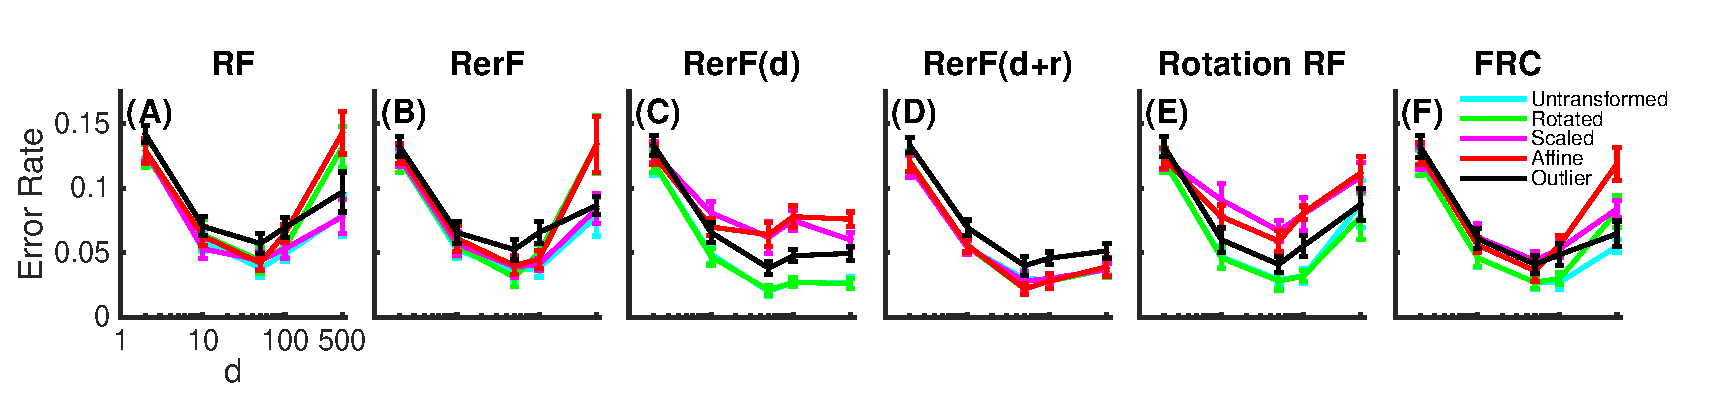
\includegraphics[width=\columnwidth]{../Figures/pdf/Fig5_robustness}}
\caption{The utility of supplementing RerF with supervised projections and rank transforming the data prior to inducing trees (see section \ref{section: additions} for details). The effect of various transformations on classification performance of RF, RerF, RerF(d), RerF(d+r), and RotRF for the Trunk simulation are shown in panels A-E, respectively. Panel D shows that RerF(d+r), which supplements RerF with supervised projections, and passes the data to ranks, is more robust to affine transformations than the other methods.}
\label{robustness}
\end{center}
\vskip -0.2in
\end{figure}

\begin{figure}[ht]
\vskip 0.2in
\begin{center}
\centerline{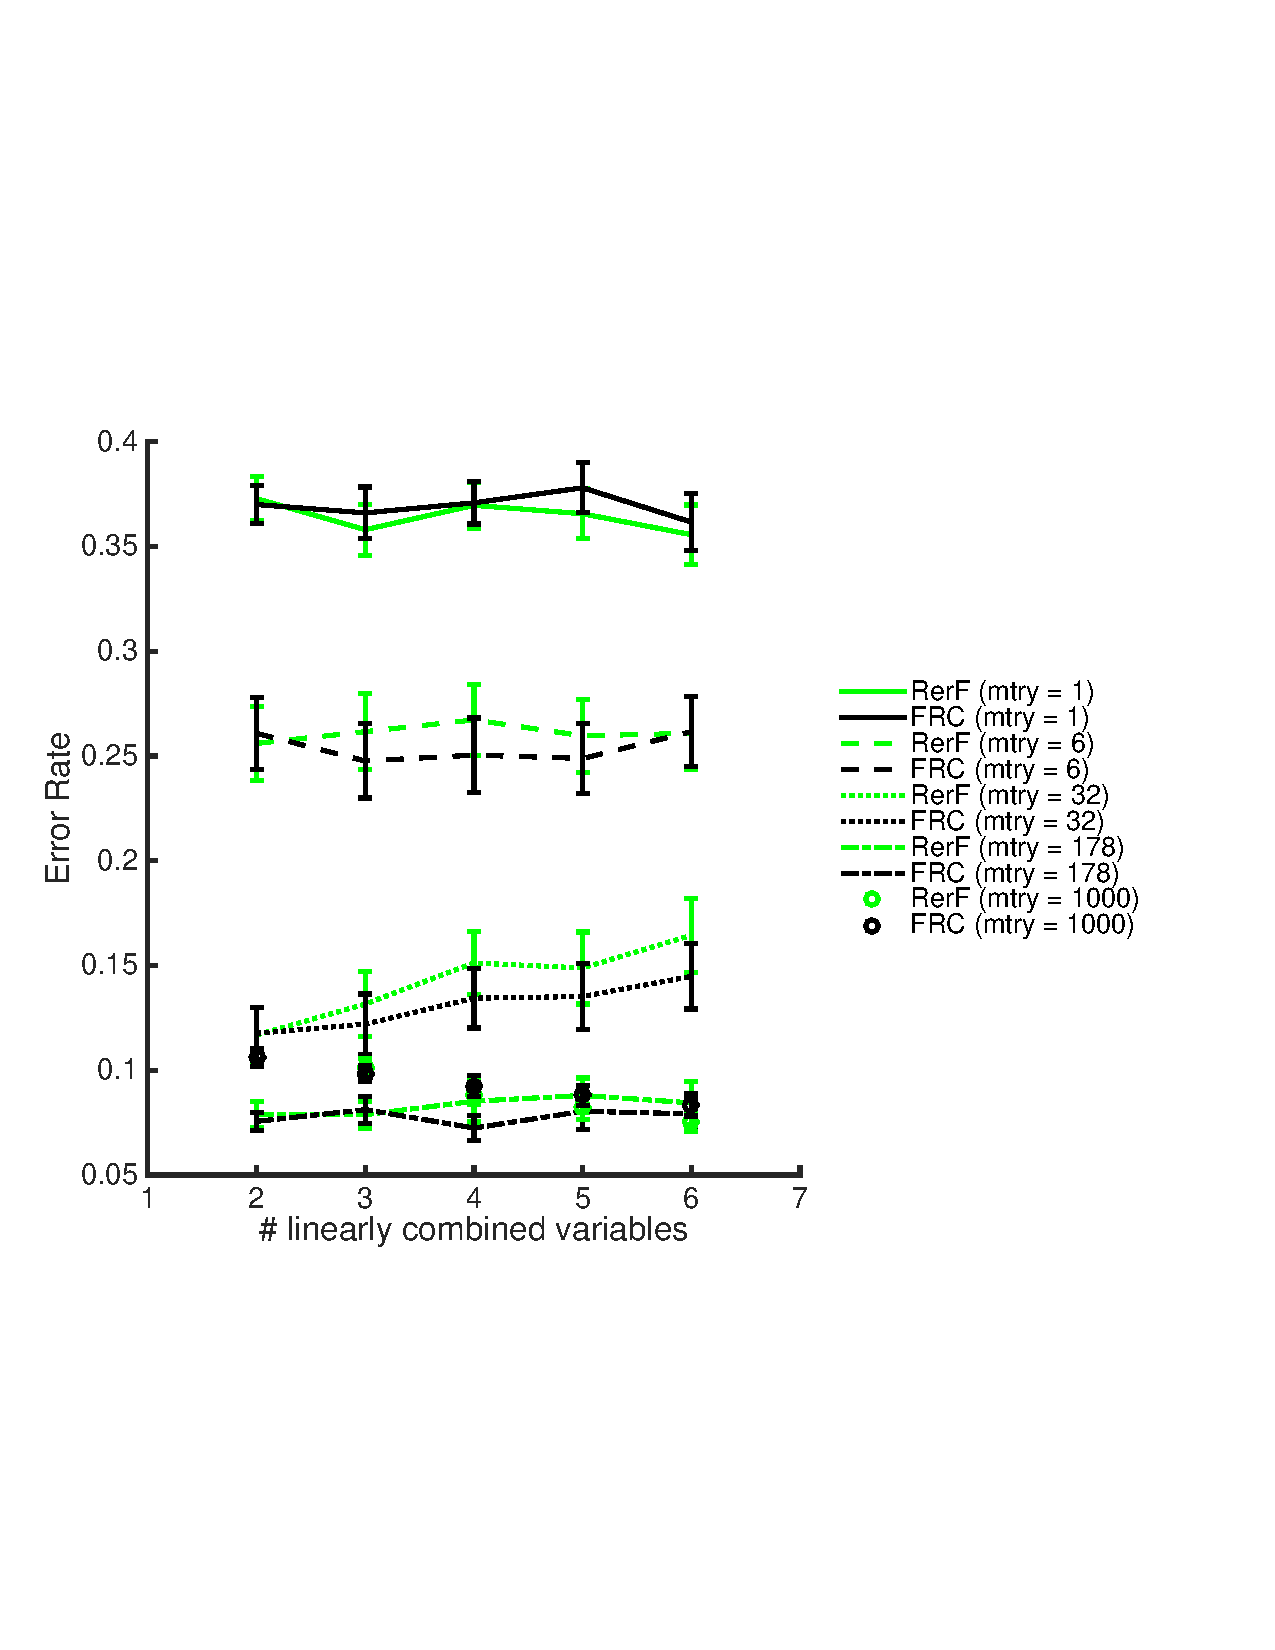
\includegraphics[width=\columnwidth]{../Figures/pdf/error_vs_sparsity}}
\caption{Error rate as a function of density of random projections and number of random projections sampled}
\label{robustness}
\end{center}
\vskip -0.2in
\end{figure}

\section{Conclusion and Future Work}

We have proposed novel methods for constructing decision forests, which we call RerFs. We view these methods as special cases of a more general random projection forest, which include Breiman's original Forest-IC and Forest-RC, as well as previously proposed oblique decision forests. We have demonstrated in simulations that RerFs are especially well-suited for classification problems in which axis-parallel splits are suboptimal, and at the same time, have a large number of irrelevant features relative to relevant ones. This could explain RerF's excellent empirical performance on a suite of over 100 benchmark datasets, as real data often has the properties just described. Moreover, RerF, unlike other oblique decision forests, preserves the time and space complexity of Forest-IC, and is only marginally sensitive to scaling. Lastly, we propose two additional modifications. One involves supplementing sparse random projections with a particular form of fast supervised projections in the construction of candidate split directions. The other involves passing the data to ranks with the goal of making the classifier more robust to outliers.

Much work is still to be done with our proposed methods. The simplicity of RerFs suggest that they will be amenable to theoretical investigation, extending the work of Biau et al. (2008) to the RerF setting \cite{biau2008}. Moreover, we hope that theoretical investigations will yield more insight into which distributions $f_A(\mc{D}_n)$ will be optimal under different distributional settings, both asymptotically and under finite sample assumptions. Even under the currently proposed $f_A(\mc{D}_n)$, our implementation has room for improvement. Although it has the same space and time complexity as RF, we will determine explicit constants, and improve our implementation accordingly. Indeed, our current implementation is a proof-of-concept MATLAB implementation. We will utilize recent GPU and semi-external memory methods to significantly speed up RerF \cite{zheng15flashgraph}. As with all decision forests, multiclass classification is but one exploitation task they can be used for; therefore, we will also extend this work to enable regression, density estimation, clustering, and hashing. We will provide open source code to enable more rigorous and extended analyses by the machine learning community.

\section*{Acknowledgements}

This work is graciously supported by the Defense Advanced Research Projects Agency (DARPA) SIMPLEX program through SPAWAR contract N66001-15-C-4041 and DARPA GRAPHS N66001-14-1-4028.

\bibliography{RandomerForest}
\bibliographystyle{IEEEtran}

\end{document} 
